\section{Usability-Analyse}
\begin{frame}
	\frametitle{Vorgehensweise}
	\begin{itemize}
		\item[1] Grobe Seitenauswahl 
		\item[2] Fragebogen ausfüllen
		\item[3] Fazit pro Seite
		\item[4] Stetige Re-Evaluation während Implementierung
	\end{itemize}
\end{frame}

\begin{frame}
	\frametitle{Usability Analyse}
	Basierend auf der Idee werden Konkurrenten bestimmt
	\begin{itemize}
		\item Absolut Vodka
		\item Alnatura
		\item Bacardi
		\item Fritz Kola
		\item Mate Drinks
		\item MyMuesli
	\end{itemize}
\end{frame}


\subsection{Positiv Beispiel}
\begin{frame}
	\frametitle{Beispiel Absolut I}
	\begin{figure}
	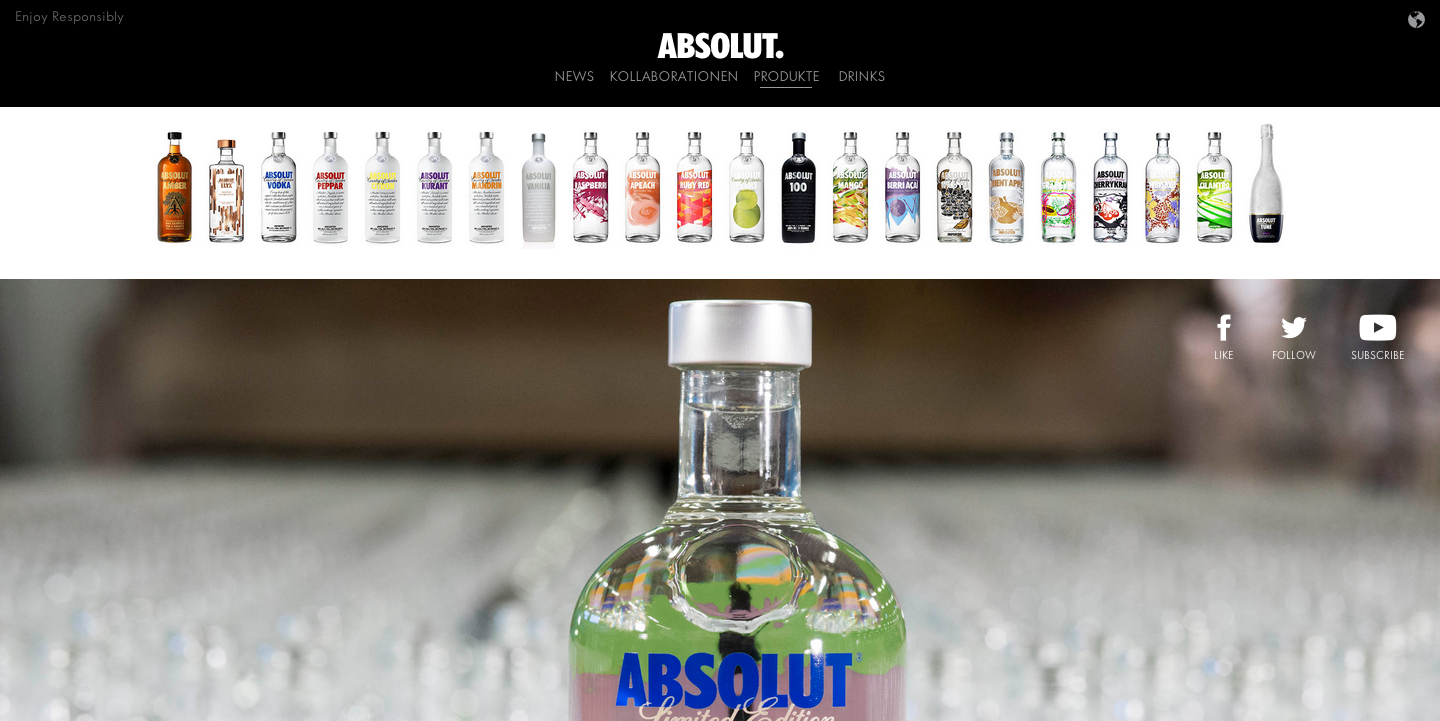
\includegraphics[scale=0.2]{bilder/absolut.png}
	\caption[Screenshot - Absolut Vodka]{Screenshot - Absolut Website}
	\label{labelname}
	\end{figure}
\end{frame}

\begin{frame}\frametitle{Beispiel Absolut II}
	\begin{tabular}{lll}
	  Kriterium & Punkte & Kommentar \\
  	  Aktualität & 9 & Blog mit aktuellen (nicht täglich) Einträgen; aktuelle Produktlinie \\
 	\end{tabular}
\end{frame}

\subsection{Negativ Beispiel}
\begin{frame}
	\frametitle{MateDrinks}
	\begin{figure}
	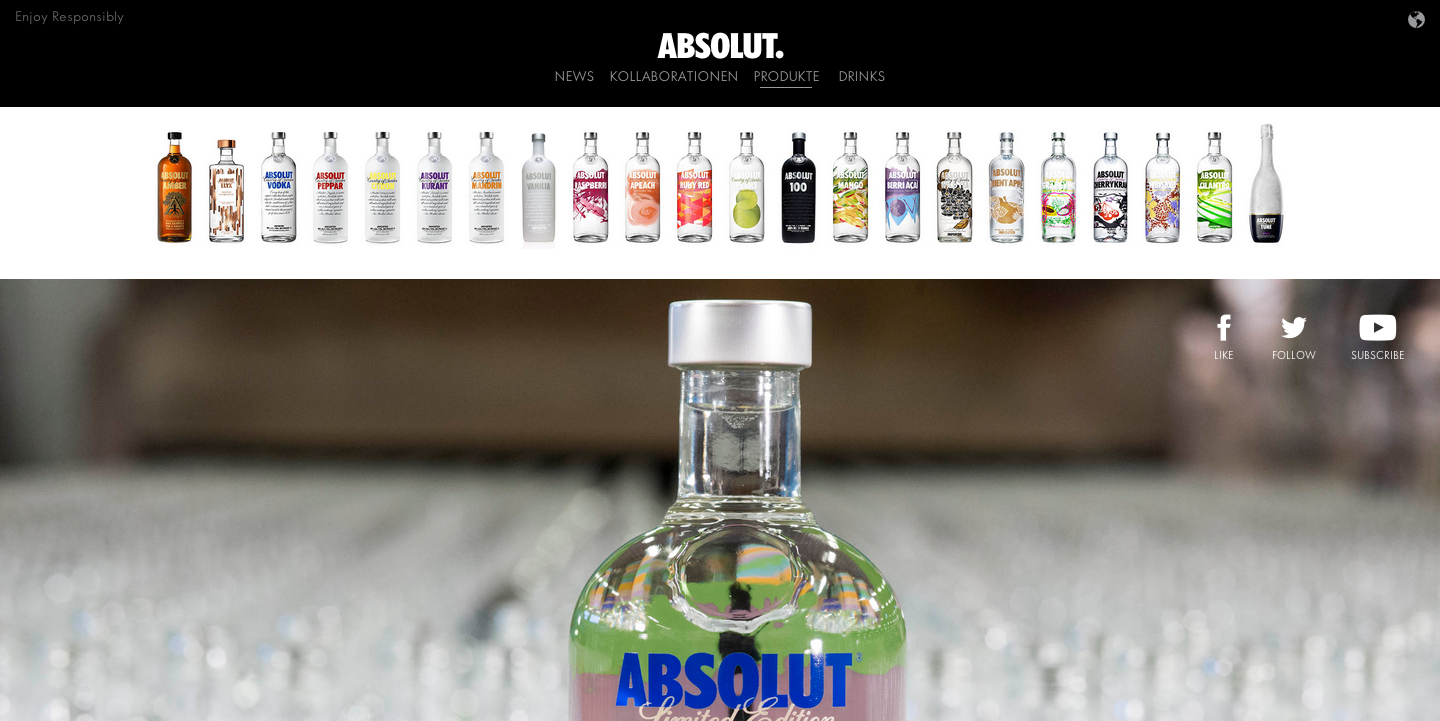
\includegraphics[scale=0.2]{bilder/absolut.png}
	\caption[Screenshot - Absolut Vodka]{Screenshot - Absolut Website}
	\label{labelname}
	\end{figure}
\end{frame}

\subsection{Fazit}
\begin{frame}
	\frametitle{Fazit}
	\begin{itemize}
		\item Bla1
		\item Bla2
		\item Bla3
	\end{itemize}
\end{frame}

